\documentclass[reqno]{amsart}


\usepackage[utf8]{inputenc}
\usepackage{amsmath}
\usepackage{amssymb}
\usepackage{hyperref}
\hypersetup{
    colorlinks=true,
    linkcolor=magenta,
    citecolor=magenta,
    filecolor=magenta,      
    urlcolor=cyan,
    pdftitle={Look and Say Sequences},
    pdfpagemode=FullScreen,
    }
\usepackage{verbatim}
\usepackage{dsfont}
\usepackage{enumerate}
\usepackage[all]{xy}
\usepackage[mathscr]{eucal}
\usepackage[usenames]{color}
\usepackage{amsthm}
\usepackage{stmaryrd}
\usepackage{amsfonts}
\usepackage{latexsym}
\usepackage{amscd}
\usepackage{graphicx}
\usepackage{setspace}
\usepackage{wasysym}
\usepackage[usenames,dvipsnames]{xcolor}
\usepackage{tikz}
\usepackage{tikz-cd}
\usepackage{todonotes}

\usepackage{color, colortbl}
\definecolor{Gray}{gray}{0.9}

\makeatletter


\newtheorem{theorem}{Theorem}[section]
\newtheorem{problem}{Problem}
\newtheorem{question}[theorem]{Question}
\newtheorem{iTheorem}{Theorem}
\newtheorem{lemma}[theorem]{Lemma}
\newtheorem{proposition}[theorem]{Proposition}
\newtheorem{corollary}[theorem]{Corollary} 
\theoremstyle{definition}  
\newtheorem{definition}[theorem]{Definition}
\newtheorem{example}[theorem]{Example}
\newtheorem{exercise}[theorem]{Exercise}
\newtheorem{conjecture}[theorem]{Conjecture}  
\newtheorem{remark}[theorem]{Remark}
\newtheorem{note}[theorem]{Note}
\renewcommand{\theiTheorem}{\Alph{iTheorem}}

\@addtoreset{equation}{section}
\def\theequation{\arabic{section}.\arabic{equation}}


%%%%%%%%%%%%%%% symbols shorthand %%%%%%%%%%%  
\newcommand{\Z}{\mathbb{Z}}
\newcommand{\R}{\mathbb{R}}
\newcommand{\N}{\mathbb{N}}
\newcommand{\C}{\mathbb{C}}
\newcommand{\ab}{\text{ab}}
\newcommand{\red}[1]{{\color{red}{#1}}}
\newcommand{\blue}[1]{{\color{blue}{#1}}}



\hyphenation{theo-re-ti-cal group-theo-re-ti-cal
semi-sim-ple al-geb-ras di-men-sions sim-ple ob-jects
equi-va-lent pro-per-ties ca-te-go-ries ques-tion mo-dule
e-print auto-equi-valence equi-va-ri-an-ti-za-tion}

\allowdisplaybreaks

\newcommand{\shift}{7}

\begin{document}

\title{An introduction to nonstandard look and say sequences}


\author[Comes]{Jonathan Comes}
\email{jcomes@collegeofidaho.edu}

\date{\today}


%\subjclass[2010]{17B10, 18D10}
%\thanks{2010 {\it Mathematics Subject Classification}: 17B10, 18D10.}


% \begin{abstract}

% \end{abstract}

\maketitle  

%\tableofcontents

\section{Introduction}\label{section: Introduction}

Here is an example of a standard look and say sequence:
\begin{equation}\label{equation: standard las 111}
    % 1, 11, 21, 1211, 111221, 312211, 13112221, 1113213211,\ldots
    % 222, 32, 1312, 11131112, 31133112, 1321232112,\ldots
    111\to 31\to 1311\to 111321\to 31131211\to 132113111221\to\cdots
\end{equation}
Roughly speaking, the rule for generating the sequence is ``say what you see''. More precisely, the sequence above starts with the \emph{seed} 111. When we look at 111 we see \red{three} \blue{1}'s and thus the next term is \red{3}\blue{1}. Looking at 31 we see \red{one} \blue{3} followed by \red{one} \blue{1}, so the next term is \red{1}\blue{3}\red{1}\blue{1}. Continuing, from 1311 we see \red{one} \blue{1}, \red{one} \blue{3}, and then \red{two} \blue{1}'s, which gives the next term \red{1}\blue{1}\red{1}\blue{3}\red{2}\blue{1}. Eventually the terms in the sequence above appear to be growing, which brings us to the following:

\begin{problem}\label{problem: growth rate}
    Determine the growth rate of a given look and say sequence.
\end{problem}

The solution to Problem \ref{problem: growth rate} for the sequence (\ref{equation: standard las 111})\footnote{And every other standard look and say sequence!}
 is given by John Conway in \cite{Conway}. In order to describe Conway's solution let us consider the number of digits (i.e.~the \emph{length}) of each term in (\ref{equation: standard las 111}):
\begin{equation*}
    3, 2, 4, 6, 8, 12,\ldots
\end{equation*}
According to Conway, the ratios of those lengths approach what is now called \emph{Conway's constant}:
\begin{equation*}\label{Conway constant}
    1.303577269\ldots%0342963912570991121525498\ldots
\end{equation*}
In other words, on average each term in (\ref{equation: standard las 111}) is approximately $30\%$ longer than the previous term. Conway's constant is remarkable in that it is the largest real root of the following irreducible polynomial:
\begin{align*}
    & \lambda^{71} - \lambda^{69} - 2 \lambda^{68} - \lambda^{67} + 2 \lambda^{66} + 2 \lambda^{65} + \lambda^{64} - \lambda^{63} - \lambda^{62} - \lambda^{61} - \lambda^{60} - \lambda^{59} + 2 \lambda^{58} 
    \\ &
    + 5 \lambda^{57} + 3 \lambda^{56} - 2 \lambda^{55} - 10 \lambda^{54} - 3 \lambda^{53} - 2 \lambda^{52} + 6 \lambda^{51} + 6 \lambda^{50} + \lambda^{49} + 9 \lambda^{48} - 3 \lambda^{47} 
    \\ &
    - 7 \lambda^{46} - 8 \lambda^{45} - 8 \lambda^{44} + 10 \lambda^{43} + 6 \lambda^{42} + 8 \lambda^{41} - 5 \lambda^{40} - 12 \lambda^{39} + 7 \lambda^{38} - 7 \lambda^{37} + 7 \lambda^{36} 
    \\ &
    + \lambda^{35} - 3 \lambda^{34} + 10 \lambda^{33} + \lambda^{32} - 6 \lambda^{31} - 2 \lambda^{30} - 10 \lambda^{29} - 3 \lambda^{28} + 2 \lambda^{27} + 9 \lambda^{26} - 3 \lambda^{25} 
    \\ &
    + 14 \lambda^{24} - 8 \lambda^{23} - 7 \lambda^{21} + 9 \lambda^{20} + 3 \lambda^{19} - 4 \lambda^{18} - 10 \lambda^{17} - 7 \lambda^{16} + 12 \lambda^{15} + 7 \lambda^{14} + 2 \lambda^{13} 
    \\ &
    - 12 \lambda^{12} - 4 \lambda^{11} - 2 \lambda^{10} + 5 \lambda^{9} + \lambda^{7} - 7 \lambda^{6} + 7 \lambda^{5} - 4 \lambda^{4} + 12 \lambda^{3} - 6 \lambda^{2} + 3 \lambda - 6
\end{align*}
The surprisingly high degree of the polynomial above indicates that the underlying mathematical structure of these look and say sequences may be more complicated than the simple ``say what you see'' rule might initially lead you to believe. Indeed, Conway discovered a beautiful structure of these look and say sequences that is ultimately governed by a linear transformation of a 92-dimensional vector space! 

The purpose of this article is definitely not to attempt to improve upon Conway's delightful explanation of his methods and results in \cite{Conway}. Instead, we hope to explain how Conway's methods and results can be generalized to other (nonstandard) look and say sequences. Many variations of look and say sequences have already been explored (see e.g.~\cite{brier2020stuttering,brier2020lookandsay}, \cite{Matin}, \cite{Morrill}, \cite{SauerbergShu}). We will be interested in look and say sequences that arise from various (nonstandard) number systems. For example, one could use Roman numerals\footnote{Conway once said that Roman numeral look and say sequences correspond to a degree 20 polynomial (see \cite{Conway-numberphile}). I would love for someone to show me how to prove this.} 
to generate the following look and say sequence:
\begin{equation*}
    \text{I$\to$ II$\to$ III$\to$ IIII$\to$ IVI$\to$ IIIVII$\to$ IIIIIVIII$\to$ VIIVIIII}\to\cdots
\end{equation*}

\subsection{Outline} In Section \ref{section::negafibnary look and say} we will completely describe the structure of all look and say sequences for a particular nonstandard number system we call the \emph{negafibnary number system}, which is related to Fibonacci numbers. The structure in the negafibnary case is much simpler than the standard case worked out by Conway. Along the way we will compare the negafibnary results to the analogous results in \cite{Conway}. Moreover, we will provide exercises so that the reader can work out the details for a third case coming from the so-called \emph{negabinary number system}.




\section{Negafibnary look and say sequences}\label{section::negafibnary look and say}

\subsection{The negafibnary number system} \label{subsection: negafibnary}
In this subsection we will explain how to create a binary number system from Fibonacci numbers using something called a \emph{Zeckendorf representation}. First, recall the definition of the Fibonacci sequence:
\begin{equation*}\label{equation: Fibonacci defintion}
    F_0 = 0, \quad F_1 = 1, \quad F_{n+1} = F_{n} + F_{n-1}.
\end{equation*}
Although Fibonacci numbers are usually considered with nonnegative index, we always have $F_{n-1}=F_{n+1}-F_n$ which allows use to extend Fibonacci numbers to negative indexes. Indeed, $F_{-1}=F_1-F_0=1-0=1$,  $F_{-2}=F_0-F_{-1}=0-1=-1$, and so on. Here is the extended Fibonacci sequence:
\begin{equation*}
    \ldots,34,-21,13,-8,5,-3,2,-1,1,0,1,1,2,3,5,8,13,21,34,\ldots
\end{equation*}
Note that $F_{-k}=(-1)^{k+1}F_k$ for all $k$. 

Zeckendorf's Theorem states that every positive integer can be written uniquely as a sum of nonadjacent Fibonacci numbers (see \cite{Zeckendorf}). For our purposes, we will use the following negative index analog of Zeckendorf's Theorem due to Bunder:

\begin{theorem}\label{theorem: Bunder-Zeckendorf} \cite{Bunder} 
    Every nonzero integer can be written uniquely in the form $\sum\limits_{j=1}^k b_jF_{-j}$ where each $b_j\in\{0,1\}$, $b_k=1$, and $b_{j+1}=0$ whenever $b_j=1$.
\end{theorem}  

If we interpret the $b_j$'s in the theorem above as bits we obtain a nonstandard binary representation of the integers. More precisely, we will write the binary string $b_k\cdots b_2b_1$ for the integer $n=\sum\limits_{j=1}^k b_jF_{-j}$. We will call $b_k\cdots b_2b_1$ the \emph{negafibnary representation} of $n$.  For example, $101$ is the negafibnary representation of the integer $F_{-3}+0\cdot F_{-2}+F_{-1}=2+0+1=3$. Similarly, $10010$ is the negafibnary representation of $F_{-5}+F_{-2}=5-1=4$. Using this terminology, Theorem \ref{theorem: Bunder-Zeckendorf} says that every integer has a unique negafibnary representation (with no adjacent 1's). The following table shows the negafibnary representation for the first few nonnegative integers:
\[\begin{array}{cccccccccc}
    0 & 1 &  2  &  3  &   4   &   5   &   6   &   7   &   8   &    9    \\ \hline
    0 & 1 & 100 & 101 & 10010 & 10000 & 10001 & 10100 & 10101 & 1001010 
\end{array}\]



\subsection{A negafibnary look and say sequence}\label{subsection: negative Zeckendorf las}
Using negafibnary representations gives us a new way to \emph{say} what we see when generating a look and say sequences. For example, if we look at $1111$ then we see \red{four} \blue{1}'s. Since the negafibnary representation of four is 10010 we would say \red{10010}\blue{1}. As in the standard case, repeatedly applying this say-what-you-see operation will generate a look and say sequence. 

Consider the look and say sequence starting with the seed 0. First, we see \red{one} \blue{0} so the next term is \red{1}\blue{0}. From 10 we see \red{one} \blue{1} and \red{one} \blue{0} so the next term is \red{1}\blue{1}\red{1}\blue{0}. Now, looking at 1110 we see \red{three} \blue{1}'s followed by \red{one} \blue{0}; since the negafibnary representation of three is 101, the next term will be \red{101}\blue{1}\red{1}\blue{0}. Continuing on in this manner gives us the following look and say sequence:
\begin{equation}\label{equation: negafibnary las with seed 0}
    0\to 10\to 1110\to 101110\to 1110101110\to 1011101110101110\to\cdots
\end{equation}
You might be able to spot a pattern by inspecting the terms above. Following Conway, in order to fully understand the structure of the sequence we should ``split'' it into smaller sequences. We explain how to do so in \S\ref{subsection: splitting}. First, we introduce another example of a nonstandard look and say sequence. 

\subsection{The negabinary case}\label{subsection: negabinary}
Suppose $b_0,b_1,\ldots,b_k\in\{0,1\}$ are bits with $b_k=1$. We call $b_k\cdots b_1b_0$ the \emph{negabinary representation} of the integer $n=\sum\limits_{j=0}^kb_j(-2)^j$. For example, $6=(-2)^4+(-2)^3+(-2)^1$ so the negabinary representation of $6$ is $11010$. It turns out that every integer has a unique negabinary representation. As we develop the theory of negafibnary look and say sequences, we will explore the analogous structure of negabinary look and say sequences in exercises. 

\begin{exercise}
    Find the negabinary representation for each of $1, 2, 3,\ldots, 10$.
\end{exercise}

\begin{exercise}\label{Exercise: negabinary las with seed 0}
    Write the first several terms of the negabinary look and say sequence starting with seed 0.
\end{exercise}

\subsection{Splitting into elements}\label{subsection: splitting}
Consider the following negafibnary look and say sequences with seeds $x=0$, $y=10$, and $z=010$:
\begin{equation*}
\begin{array}{cccccccccccccc}
x &=& \red{0}   &\to& \red{10}    &\to& \red{1110}    &\to& \red{101110}      &\to& \cdots\\
y &=& \blue{10} &\to& \blue{1110} &\to& \blue{101110} &\to& \blue{1110101110} &\to& \cdots\\
z &=& \red{0}\blue{10} &\to& \red{10}\blue{1110} &\to& \red{1110}\blue{101110} &\to& \red{101110}\blue{1110101110} &\to& \cdots
\end{array}
\end{equation*}
Notice that each term of the look and say sequence with seed $z$ can be obtained by concatenating the corresponding terms from seed $x$ to the left of the terms from seed $y$. When this happens we say that $z$ \emph{splits} and write $z=x.y$. Note that the splitting allows us to completely determine the sequence with seed $z$ from the sequences with smaller seeds $x$ and $y$. This reduction is the key to Conway's method for analyzing look and say sequences. 

When reducing look and say sequences via splitting, one must be careful that the splitting occurs for \emph{all} of the terms in a look and say sequence. For example, consider the standard look and say sequences with seeds $x=3$, $y=2$, and $z=32$:
\begin{equation*}
\begin{array}{cccccccccccccc}
x &=& \red{3}  &\to& \red{13}  &\to& \red{1113}  &\to& \red{3113}   &\to& \red{132113}  &\to& \cdots\\
y &=& \blue{2} &\to& \blue{12} &\to& \blue{1112} &\to& \blue{3112}  &\to& \blue{132113} &\to& \cdots\\
z &=& \red{3}\blue{2} &\to& \red{13}\blue{12} &\to& \red{1113}\blue{1112} &\to& \red{3113}\blue{3112} &\to& 1321232112&\to& \cdots
\end{array}
\end{equation*}
While the first few terms of sequence from seed $z$ is obtained by concatenating those from $x$ and $y$, eventually we find a term from $z$, namely $1321232112$, which differs from the concatenation of the corresponding terms from $x$ and $y$, namely $\red{132113}\blue{132113}$. Thus, in the standard case $32\not=3.2$. 


% Let us write $LS$ for the say-what-you-see operation so that the arrow notation used in all the look and say sequences above can be viewed as $x\to LS(x)$. For example, in the standard case $LS(111)=31$ and $LS(31)=1311$ (compare with (\ref{equation: standard las 111})). On the other hand, in the negafibnary case we have $LS(1110)=101110$ (compare with (\ref{equation: negafibnary las with seed 0})). Note that we are abusing notation a bit since we are writing $LS$ for both the standard case and the negafibnary case, but we expect the distinction will be clear from context.

% Given strings of digits $x$ and $y$ we will simply write $xy$ for their concatenation (i.e.~write $x$ to the left of $y$). For example, if $x=10$ and $y=11100$ we have $xy=1011100$. Note that we are straying from the usual convention in that $xy$ does not refer to multiplication. The reason for this is that multiplication is not the important operation here, concatenation is! 

% Now, we say a string of digits $z=xy$ \emph{splits as} $z=x.y$ if $LS^k(z)=LS^k(x)LS^k(y)$ for all $k\geq 0$. In other words, $z=xy$ splits as $z=x.y$ if the entire look and say sequence with seed $z$ is the same as the term-by-term concatenation of the look and say sequences with seeds $x$ and $y$. For example, consider the negafibnary look and say sequences with seeds $x=0$, $y=10$, and $z=xy=010$:
% \begin{equation*}
% \begin{array}{cccccccccccccc}
% x &=& 0  &\to& 10   &\to& 1110   &\to& 101110     &\to& \cdots\\
% y &=& 10 &\to& 1110 &\to& 101110 &\to& 1110101110 &\to& \cdots\\
% z &=& 010 &\to& 101110 &\to& 1110101110 &\to& 1011101110101110 &\to& \cdots
% \end{array}
% \end{equation*}

\begin{problem}\label{problem: splitting theorem}
    Determine precisely when and how look and say sequences split.
\end{problem}

The solution to Problem \ref{problem: splitting theorem} for standard look and say sequences is Conway's Splitting Theorem (see \cite{Conway}). Before providing the solution in the negafibnary case, it will be convenient to introduce a bit of notation. Let us write $xy$ for the concatenation of $x$ and $y$ (i.e.~$x$ placed to the left of $y$). For example, if $x=10$ and $y=11100$ we have $xy=1011100$. Note that we are straying from the usual convention in that $xy$ does not refer to multiplication. Now we are in a good position to solve Problem \ref{problem: splitting theorem} in the negafibnary case:

\begin{theorem}\label{theorem: negafibnary splitting theorem} (Negafibnary Splitting Theorem)
    Given any binary string $z$, the corresponding negafibnary look and say sequence splits as $z=x.y$ whenever $z=xy$, the rightmost bit in $x$ is a 0, and the leftmost bit in $y$ is a 1.
\end{theorem}

\begin{proof}
    Write $x=x_0\to x_1\to x_2\to\cdots$, $y=y_0\to y_1\to y_2\to\cdots$, and finally $z=z_0\to z_1\to z_2\to\cdots$ for the relevant look and say sequences. We use induction to show that for every $k\geq 0$ we have (i) $z_k=x_ky_k$, (ii) the rightmost bit of $x_k$ is a 0, and (iii) the leftmost bit of $y_k$ is a 1. The base case is given by the hypothesis of the theorem. For the inductive step, assume (i)--(iii) hold for some $k\geq 0$. Now, since the rightmost bit of $x_k$ is 0, the last thing you see in $x_k$ will be some run of 0's, hence $x_{k+1}$ will also end with a 0. Next, since the start of $y_{k+1}$ is the negafibnary representation of the number of $1$'s on the very left of $y_k$, and every negafibnary representation of a positive integer starts with a 1, it follows that $y_{k+1}$ starts with a 1. Finally, since $x_k$ ends with a 0 and $y_k$ starts with a 1, there is no interaction between $x_k$ and $y_k$ when performing the say-what-you-see operation on $z_k=x_ky_k$. It follows that $z_{k+1}=x_{k+1}y_{k+1}$.
\end{proof}

\begin{exercise}
    Does Theorem \ref{theorem: negafibnary splitting theorem} still hold if we replace negafibnary with negabinary? Why or why not? 
\end{exercise}

Using Theorem \ref{theorem: negafibnary splitting theorem} we can completely split any binary string in the negafibnary case. For example, $111011000=1110.11000$. Some binary strings can be split more than once: $101101001100=10.110.100.1100$. More generally, any binary string splits into strings consisting of some 1's followed by some 0's. To state this a bit more precisely, let us write $x^n$ for the concatenation of the string $x$ with itself $n$ times. Then every binary string in the negafibnary case splits into strings of the form 
\begin{equation}\label{binary elements}
    1^m0^n = \underbrace{1\cdots 1}_{m}\underbrace{0\cdots 0}_{n}
\end{equation}
where $m$ and $n$ are nonnegative integers. 

Strings that cannot be split are called \emph{elements}. An arbitrary string is a \emph{compound} of the elements it splits into. We have shown that the elements in the negafibnary case are precisely the binary strings (\ref{binary elements}). This terminology goes back to Conway's work in \cite{Conway}. Conway's splitting theorem for the standard case is more complicated than Theorem \ref{theorem: negafibnary splitting theorem}, and thus the elements in the standard case do not possess a simple form like (\ref{binary elements}). However, Conway found 92 \emph{common elements} that appear in almost every look and say sequence; he named these common elements after the 92 naturally-occurring elements hydrogen, helium,$\ldots$, uranium. 

Since every string splits into elements, and the say-what-you-see operation on the elements do not interact with one another, the structure of any look and say sequence is completely determined by the elements that appear in the sequence. For example, consider the sequence (\ref{equation: negafibnary las with seed 0}). Every term after the initial seed is a compound of the two elements $10$ and $1110$. Thus we will be able to solve Problem \ref{problem: growth rate} for sequence (\ref{equation: negafibnary las with seed 0}) by analyzing the say-what-you-see operation on just those two elements. 

We say an element appears \emph{frequently} in a look and say sequence if that element appears in infinitely many of the terms. For example, the only elements that appear frequently in (\ref{equation: negafibnary las with seed 0}) are $10$ and $1110$. Determining the frequent elements in a look and say sequence is a crucial step towards solving Problem \ref{problem: growth rate}.

\begin{problem}\label{problem::find frequent elements}
    Given a look and say sequence equipped with a splitting theorem, determine all the elements that appear frequently. 
\end{problem}


\begin{exercise}\label{Exercise: negabinary elements from seed 0}
    Find all the elements that appear frequently in the negabinary look and say sequence from Exercise \ref{Exercise: negabinary las with seed 0}. 
\end{exercise}

\subsection{Decay and decay matrices}\label{subsection::decay}
Continuing with the chemical terminology, if the say-what-you-see operation takes $x\to y$ then we say the compound $x$ \emph{decays} into $y$. For example, in the negafibnary case we have $0\to 10$, so $0$ decays into $10$. Now let 
\begin{equation}\label{negafibnary two common elements}
    e_1=10\quad\text{and}\quad e_2=1110.
\end{equation} 
Then $e_1=10\to 1110=e_2$ and $e_2=1110\to 101110=e_1e_2$. Thus $e_1$ decays into $e_2$, and $e_2$ decays into $e_1e_2$.

\begin{exercise}\label{Exercise: negabinary decay from seed 0}
    Determine the negabinary decay of each element from Exercise \ref{Exercise: negabinary elements from seed 0}.
\end{exercise}

Suppose $e_1,\ldots,e_k$ is a collection of elements such that each $e_j$ decays into a compound of some of the $e_i$'s. To these elements we associate a $k$-dimensional vector space of column vectors called the \emph{compound space}. Given a compound of these elements, the corresponding \emph{compound vector} is the column vector whose $i$th entry is the number of times $e_i$ appears in the compound. For example, consider the last string written in the sequence (\ref{equation: negafibnary las with seed 0}). Keeping with (\ref{negafibnary two common elements}), that string is a compound of 2 $e_1$'s and 3 $e_2$'s, so the corresponding compound vector is 
$\begin{pmatrix}
    2 \\ 3
\end{pmatrix}$.

Returning to the general setup with $k$ elements, the \emph{decay matrix} is the $k\times k$ matrix whose $i,j$-entry is the number of times $e_i$ occurs in the decay of $e_j$. In other words, the $j$th column is the compound vector corresponding to the decay of $e_j$. For example, with (\ref{negafibnary two common elements}) in the negafibnary case the decay matrix is 
\begin{equation}\label{negafibnary 2x2 decay matrix}
    % D = 
    \begin{pmatrix}
        0 & 1\\
        1 & 1
    \end{pmatrix}.
\end{equation}
Indeed, the first column is 
$\begin{pmatrix}
        0 \\
        1 
\end{pmatrix} $
since  $e_1$ decays into zero $e_1$'s and one $e_2$; the second column is 
$\begin{pmatrix}
        1 \\
        1 
\end{pmatrix}$
because $e_2$ decays into one $e_1$ and one $e_2$. 

\begin{exercise}\label{exercise: negabinary decay matrix for seed 0}
    Use your answer to Exercise \ref{Exercise: negabinary decay from seed 0} to find a decay matrix for the negabinary look and say sequence from Exercise \ref{Exercise: negabinary las with seed 0}. To get started you will need to fix an order on the elements. Your matrix will depend on the order you choose. 
\end{exercise}

The decay matrix is so-named because multiplying a compound vector by the decay matrix corresponds to decaying the compound via the say-what-you-see operation. For example, we have already seen $1110101110\to 1011101110101110$ in the negafibnary case (see (\ref{equation: negafibnary las with seed 0})). The first of these compounds corresponds the vector 
$\begin{pmatrix}
    1\\ 2
\end{pmatrix}$. Multiplying by the decay matrix we get $\begin{pmatrix}
    0 & 1\\ 1 & 1
\end{pmatrix}
\begin{pmatrix}
    1\\ 2
\end{pmatrix}
=
\begin{pmatrix}
    2\\ 3
\end{pmatrix}$, which we've already seen is the compound vector for the decay compound. 
Similarly, one can check that every step in the following sequence is obtained via left multiplication by the decay matrix (\ref{negafibnary 2x2 decay matrix}):
\begin{equation}\label{negafibnary decay sequence in coordinates}
    \begin{pmatrix}
        1\\ 0
    \end{pmatrix}
    \mapsto
    \begin{pmatrix}
        0\\ 1
    \end{pmatrix}
    \mapsto
    \begin{pmatrix}
        1\\ 1
    \end{pmatrix}
    \mapsto
    \begin{pmatrix}
        1\\ 2
    \end{pmatrix}
    \mapsto
    \begin{pmatrix}
        2\\ 3
    \end{pmatrix}
    \mapsto
    \begin{pmatrix}
        3\\ 5
    \end{pmatrix}
    \mapsto
    \cdots
\end{equation}
Note that the first 5 vectors in (\ref{negafibnary decay sequence in coordinates}) are the compound vectors for the last 5 terms of (\ref{equation: negafibnary las with seed 0}). The first term of (\ref{equation: negafibnary las with seed 0}), 0, does not correspond to a compound vector in this compound space since 0 is not a compound of $e_1=10$ and $e_2=1110$. The last vector in (\ref{negafibnary decay sequence in coordinates}) tells us that the next (unwritten) term in (\ref{equation: negafibnary las with seed 0}) will be a compound of 3 $e_1$'s  and 5 $e_2$'s. Notice that all the coordinates in (\ref{negafibnary decay sequence in coordinates}) are Fibonacci numbers!

\begin{exercise}
    Find the sequence of compound vectors for the negabinary look and say sequence from Exercise \ref{Exercise: negabinary las with seed 0}. In other words, (\ref{equation: negafibnary las with seed 0}) is to (\ref{negafibnary decay sequence in coordinates}) as your answer to Exercise \ref{Exercise: negabinary las with seed 0} is to what? The coordinates in these compound vectors are the so-called \emph{Padovan numbers}.
\end{exercise}

Although the decay matrix encodes a significant amount of decay information, one cannot completely recover a look and say sequence from the corresponding decay matrix and compound vectors. This is because the compound vector of a given compound does not encode the \emph{order} in which the elements appear in a given compound. For example, the two different compounds $e_1e_2$ and $e_2e_1$ have the same compound vector 
$\begin{pmatrix}
    1 \\ 1
\end{pmatrix}$. 
However, if we are concerned with a problem that does not depend on the order of the elements, like Problem \ref{problem: growth rate}, then we can often find the solution within the structure of the decay matrix. 


\subsection{Solving Problem \ref{problem: growth rate} with an eigenvalue}
The key to solving Problem \ref{problem: growth rate} is to find eigenvalues of the decay matrix $D$.  In order to find eigenvalues we first find the characteristic polynomial\footnote{Some prefer to define the characteristic polynomial of $D$ as $\det(D-\lambda I)$. I prefer $\det(\lambda I -D)$ since it will always be a monic polynomial (i.e.~the leading coefficient will be 1). These two conventions at most differ by a multiple of $-1$. In particular, they always have the same roots


.} $\det(\lambda I - D)$. For example, the characteristic polynomial of the decay matrix (\ref{negafibnary 2x2 decay matrix}) is 
\begin{equation}\label{char poly negafibnary 2x2}
    \det\begin{pmatrix}
    \lambda & -1 \\
    -1      & \lambda - 1
    \end{pmatrix}
    =\lambda^2 - \lambda - 1.
\end{equation}
The eigenvalues of a matrix are the roots of its characteristic polynomial. The roots of (\ref{char poly negafibnary 2x2}) are $\lambda = \frac{1\pm\sqrt{5}}{2}$. In particular, the maximal real eigenvalue is the celebrated golden ratio
\begin{equation}\label{phi}
    \varphi=\frac{1+\sqrt{5}}{2} = 1.61803\ldots
\end{equation}

\begin{exercise}\label{exercise: negabinary plastic ratio as eigenvalue}
    Find the characteristic polynomial for the decay matrix from Exercise \ref{exercise: negabinary decay matrix for seed 0}. Use technology to determine the maximal real root of the characteristic polynomial. This number is the so-called \emph{plastic ratio} often denoted $\rho$.
\end{exercise}

We will show that the golden ratio is negafibnary analog of Conway's constant. In particular, the ratio of the lengths of successive terms of (\ref{equation: negafibnary las with seed 0}) approach the golden ratio, and thus solves Problem \ref{problem: growth rate} for that look and say sequence. This procedure works more generally: 

\begin{theorem}\label{theorem:: ratio of lengths approach max eigenvalue}
Given a look and say sequence whose terms are eventually compounds consisting of elements $e_1,\ldots,e_k$, the ratios of the lengths of the terms approach the maximal real eigenvalue\footnote{The fact that such an eigenvalue will always exist follows from the Perron-Frobenius Theorem.} of the corresponding $k\times k$ decay matrix. 
\end{theorem}

In the standard case, Conway's 92 elements give rise to a $92\times 92$ decay matrix. Conway's constant (\ref{Conway constant}) is the maximal real root of this decay matrix. The irreducible degree 71 polynomial given at the beginning of the introduction is a factor of the degree 92 characteristic polynomial.

Instead of proving Theorem \ref{theorem:: ratio of lengths approach max eigenvalue} in general, we will verify only the negafibnary case for the look and say sequence (\ref{equation: negafibnary las with seed 0}). However, with just a bit more linear algebra the argument given below can be generalized to give a full proof of Theorem \ref{theorem:: ratio of lengths approach max eigenvalue}. 

\bigskip

\noindent\emph{Proof of Theorem \ref{theorem:: ratio of lengths approach max eigenvalue} for (\ref{equation: negafibnary las with seed 0}).} Let $D$ denote the decay matrix (\ref{negafibnary 2x2 decay matrix}) and write $\lambda_1=\frac{1+\sqrt{5}}{2}$ and $\lambda_2=\frac{1-\sqrt{5}}{2}$ for the eigenvalues of $D$. One can show that
$v_1=\begin{pmatrix}
    1 \\
    \lambda_1
\end{pmatrix}$ and 
$v_2=\begin{pmatrix}
    1 \\
    \lambda_2
\end{pmatrix}$ are respective eigenvectors of $D$. In other words, $Dv_i=\lambda_i v_i$ for both $i=1,2$. Now, set 
$u_0=\begin{pmatrix}
    1 \\
    0
\end{pmatrix}$ and write $u_n=D^nu_0$ for each $n>0$. In other words, the sequence $u_0\mapsto u_1\mapsto u_2\mapsto\cdots$ is precisely (\ref{negafibnary decay sequence in coordinates}). Since $v_1$ and $v_2$ span all of $\R^2$ we can find $\alpha_1,\alpha_2\in\R$ such that $u_0=\alpha_1v_1+\alpha_2v_2$. The interested reader can find the exact values of $\alpha_1$ and $\alpha_2$. For our purposes, it suffices to know that such scalars exist and $\alpha_1\not=0$ (because $u_0$ is not a scalar multiple of $v_2$). The following computation is the key to the proof:

\begin{align}\label{key eigenvalue computation start}
    \frac{1}{\lambda_1^n}u_n 
    & = \frac{1}{\lambda_1^n}D^nu_0  & \text{(definition of $u_n$)}\\
    & = \frac{1}{\lambda_1^n}D^n(\alpha_1v_1+\alpha_2v_2) & \text{(definition of $\alpha_1$ and $\alpha_2$)} \\
    & = \frac{1}{\lambda_1^n}(\alpha_1\lambda_1^nv_1+\alpha_2\lambda_2^nv_2) & \text{(definition of eigenvector)}\\
    & = \alpha_1v_1+\alpha_2\left(\frac{\lambda_2}{\lambda_1}\right)^nv_2 \\
    \label{key eigenvalue computation end}
    & \to \alpha_1v_1\quad\text{as }n\to\infty & \text{(since $|\lambda_1|>|\lambda_2|$)}
\end{align}
To connect the computation above to the statement of the theorem we let $\ell$ denote the vector whose coordinates are the lengths of the elements $e_1=10$ and $e_2=1110$. More precisely, we have 
$\ell=
\begin{pmatrix}
    2 \\
    4
\end{pmatrix}$. Then the length of any compound corresponding to compound vector $u$ is given by the dot product $u\cdot\ell$. Thus, the ratio of lengths of successive terms of (\ref{equation: negafibnary las with seed 0}) is given by $\dfrac{u_{n+1}\cdot\ell}{u_n\cdot\ell}$. We can use the computation above to determine the limit of this ratio:
\begin{equation*}
    \dfrac{u_{n+1}\cdot\ell}{u_n\cdot\ell} = \lambda_1\left(\dfrac{\frac{1}{\lambda_1^{n+1}}u_{n+1}\cdot\ell}{\frac{1}{\lambda_1^{n}}u_n\cdot\ell}\right)\to\lambda_1\left(\dfrac{\alpha_1v_1\cdot\ell}{\alpha_1v_1\cdot\ell}\right)=\lambda_1\quad\text{as }n\to\infty.
\end{equation*}
~\hfill$\Box$

\begin{exercise}
    Mimic the argument above to prove that the ratios of the lengths of terms in the negabinary look and say sequence from Exercise \ref{Exercise: negabinary las with seed 0} approach the plastic ratio from Exercise \ref{exercise: negabinary plastic ratio as eigenvalue}.
\end{exercise}

\subsection{Abundances} \label{subsection: abundances}
Since Problem \ref{problem: growth rate} can be solved using the largest real eigenvalue of a decay matrix, it is natural to ask what the corresponding eigenvector tells us about the look and say sequence. We will see that eigenvectors can be used to solve the following problems:

\begin{problem}\label{abundance of elements}
    Determine the limiting relative abundance of each element in a look and say sequence.
\end{problem}

\begin{problem}\label{abundance of digits}
    Determine the limiting relative abundance of each digit in a look and say sequence.
\end{problem}

To make Problem \ref{abundance of elements} more precise we introduce some notation for abundances. Given a column vector $u$ whose coordinates sum to $s\not=0$, we write $\ab(u)=\frac{1}{s}u$ for the \emph{abundance vector of $u$}. For example, consider the last term written in the look and say sequence (\ref{equation: negafibnary las with seed 0}), namely the compound $e_1e_2e_2e_1e_2$. The corresponding compound vector is 
$u=\begin{pmatrix}
    2 \\
    3
\end{pmatrix}$
so the abundance vector is
$\ab(u)=\frac{1}{2+3}u=\begin{pmatrix}
    0.4 \\
    0.6
\end{pmatrix}$.
Note that the coordinates of $\ab(u)$ are exactly the relative abundances of the elements in the compound: $40\%$ of the elements in the compound are $e_1$ and $60\%$ are $e_2$.  Thus, to solve Problem \ref{abundance of elements} is to find the limit of the abundance vectors for a given look and say sequence. The following theorem explains how to find such a limit. 

\begin{theorem}\label{theorem:: abundance of elements approach max eigenvector}
Given a look and say sequence whose terms are eventually compounds consisting of elements $e_1,\ldots,e_k$, the corresponding sequence of abundance vectors approach $\ab(v)$ where $v$ is any eigenvector of the decay matrix with maximal real eigenvalue. 
\end{theorem}

Before proving Theorem \ref{theorem:: abundance of elements approach max eigenvector} we will see how it can be used to give explicit solutions to both Problem \ref{abundance of elements} and Problem \ref{abundance of digits} in the negafibnary case. 
% Afterwards we will provide a proof of Theorem \ref{theorem:: abundance of elements approach max eigenvector} for the negafibnary case.

Consider the negafibnary look and say sequence (\ref{equation: negafibnary las with seed 0}). Taking the abundance of each vector in (\ref{negafibnary decay sequence in coordinates}) gives us the sequence of abundance vectors:
\begin{equation}\label{negafibnary abundance sequence for seed 0}
    \begin{pmatrix}
        1\\ 0
    \end{pmatrix}
    \mapsto
    \begin{pmatrix}
        0\\ 1
    \end{pmatrix}
    \mapsto
    \begin{pmatrix}
        0.5\\ 0.5
    \end{pmatrix}
    \mapsto
    \begin{pmatrix}
        0.333\ldots\\ 0.666\ldots
    \end{pmatrix}
    \mapsto
    \begin{pmatrix}
        0.4\\ 0.6
    \end{pmatrix}
    \mapsto
    \begin{pmatrix}
        0.375\\ 0.625
    \end{pmatrix}
    \mapsto
    \cdots
\end{equation}
Now, we have already seen that the maximal eigenvalue of the decay matrix (\ref{negafibnary 2x2 decay matrix}) is the golden ratio $\lambda_1=\frac{1+\sqrt{5}}{2}$ and a corresponding eigenvector is 
$v_1=
\begin{pmatrix}
    1\\ \lambda_1
\end{pmatrix}$. Using the notation $\varphi=\frac{1+\sqrt{5}}{2}$ we have
\begin{equation}\label{abundance for negafibnary with seed 0}
    \ab(v_1)
    =\frac{1}{1+\varphi}
    \begin{pmatrix}
        1\\ \varphi
    \end{pmatrix}
    =\frac{1}{\varphi^2}
    \begin{pmatrix}
        1\\ \varphi
    \end{pmatrix}
    =\begin{pmatrix}
        \varphi^{-2}\\ \varphi^{-1}
    \end{pmatrix}
    =
    \begin{pmatrix}
        0.381\ldots\\ 0.618\ldots
    \end{pmatrix}.
\end{equation}
According to Theorem \ref{theorem:: abundance of elements approach max eigenvector} the limit of the sequence (\ref{negafibnary abundance sequence for seed 0}) is (\ref{abundance for negafibnary with seed 0}). In particular, abundances of elements $e_1=10$ and $e_2=1110$ in (\ref{equation: negafibnary las with seed 0}) are approaching $\varphi^{-2}\approx 0.38$ and $\varphi^{-1}\approx 0.62$ respectively. Hence, the ratio of the number of $e_2$'s to $e_1$'s occurring in (\ref{equation: negafibnary las with seed 0}) is approaching the golden ratio. This solves Problem \ref{abundance of elements} in the negafibnary case for (\ref{equation: negafibnary las with seed 0}). 

\begin{exercise}
    Solve Problem \ref{abundance of elements} in the negabinary case for the look and say sequence from Exercise \ref{Exercise: negabinary las with seed 0}. In particular, explain how the abundances of the elements are related by the plastic ratio $\rho$ (see Exercise \ref{exercise: negabinary plastic ratio as eigenvalue}).
\end{exercise}

In the standard case, the abundances of Conway's 92 common elements correspond to an eigenvector of a $92\times 92$ decay matrix. All 92 abundances are listed in The Periodic Table found in \cite{Conway}. Conway was not concerned with Problem \ref{abundance of digits}, but solving that problem is easy once we have a solution to Problem \ref{abundance of elements}. Indeed, the abundance of each digit in a look and say sequence can be determined from the abundance of each element in the look and say sequence together with the abundance of each digit in each element. More precisely, if $v$ is the limiting abundance vector for elements (the solution to Problem \ref{abundance of elements}) and $A$ is the matrix whose $j$th column lists the abundance of each digit in the $j$th element, then the product $A v$ gives the limiting abundance of each digit in the look in say sequence.

For example, consider the negafibnary look and say sequence (\ref{equation: negafibnary las with seed 0}). Since $e_1=10$ we see the abundances of 0 and 1 in $e_1$ are both $0.5$. Similarly, the abundances of 0 and 1 in $e_2=1110$ are $0.25$ and $0.75$ respectively. Packaging these abundances into a matrix $A$ and multiplying by the vector $v$ given in (\ref{abundance for negafibnary with seed 0}) gives 
\begin{equation*}\label{negafibnary abundance of digits for seed 0}
    \begin{pmatrix}
        0.5 & 0.25\\ 
        0.5 & 0.75
    \end{pmatrix}
    \begin{pmatrix}
        \varphi^{-2}\\ 
        \varphi^{-1}
    \end{pmatrix}
    =
    \begin{pmatrix}
        0.5\varphi^{-2}+0.25\varphi^{-1} \\
        0.5\varphi^{-2}+0.75\varphi^{-1}
    \end{pmatrix}
    =
    \begin{pmatrix}
        0.25+0.25\varphi^{-2} \\
        0.5+0.25\varphi^{-1}
    \end{pmatrix}
    \approx
    \begin{pmatrix}
        0.345 \\
        0.655
    \end{pmatrix}.
\end{equation*}
This gives us a solution to Problem \ref{abundance of digits} for the negafibnary look and say sequence (\ref{equation: negafibnary las with seed 0}): eventually there are approximately $34.5\%$ 0's and $65.5\%$ 1's in each term.

\begin{exercise}
    Solve Problem \ref{abundance of digits} for the negabinary look and say sequence from Exercise \ref{Exercise: negabinary decay from seed 0}.
\end{exercise}

As promised, we conclude this section with a proof of Theorem \ref{theorem:: abundance of elements approach max eigenvector}. The proof below relies on our proof of Theorem \ref{theorem:: ratio of lengths approach max eigenvalue}, which was only given for the negafibnary (\ref{equation: negafibnary las with seed 0}). The motivated reader is encouraged to generalize the following proof to the general case.  

\bigskip

\noindent\emph{Proof of Theorem \ref{theorem:: abundance of elements approach max eigenvector} for (\ref{equation: negafibnary las with seed 0}).} Let $\lambda_i, v_i, \alpha_i$, and $u_n$ be as in the proof of Theorem \ref{theorem:: ratio of lengths approach max eigenvalue}. To prove the theorem at hand, we will show $\ab(u_n)\to\ab(v_1)$ as $n\to\infty$. Note that the sum of the coordinates of any vector $u$ is given by the dot product $u\cdot{\bf 1}$ where ${\bf 1}$ is the column vector with all 1's as coordinates. Hence $\ab(u)=\frac{1}{u\cdot{\bf 1}}u$ for all $u$. Thus, using the result of computation (\ref{key eigenvalue computation start})--(\ref{key eigenvalue computation end}) we have 
\begin{equation*}
\ab(u_n)=\frac{1}{u_n\cdot{\bf 1}}u_n=\frac{1}{\lambda_1^{-n}u_n\cdot{\bf 1}}\lambda_1^{-n}u_n\to\frac{1}{\alpha_1 v_1\cdot{\bf 1}}\alpha_1 v_1=\frac{1}{v_1\cdot{\bf 1}} v_1=\ab(v_1)
\end{equation*}
as $n\to\infty$, which completes the proof. \hfill$\Box$


\subsection{Completing the chemistry} 
The elements that appear frequently (i.e.~infinitely many times) in a look and say sequence depend on the seed. For example, in the negafibnary case we know the look and say sequence (\ref{equation: negafibnary las with seed 0}) with seed 0 has two frequently occurring elements: $e_1=10$ and $e_2=1110$. On the other hand, if the seed is instead 1 we get the following look and say sequence:
\begin{equation*}\label{negafibnary las with seed 1}
1 \to 11 \to 1001 \to 11100011 \to 101110101001 \to 1110101110111011100011 \to \cdots
\end{equation*}
In addition to the elements $e_1$ and $e_2$, the elements $1, 11, 100$, and $111000$ also appear frequently in the sequence above. There are still other elements that appear frequently in other negafibnary look and say sequences, like $110$ in the following:
\begin{equation}\label{negafibnary las with seed 110}
110 \to 100110 \to 111000100110 \to 10111010111000100110 \to\cdots
\end{equation}
In fact, there exist negafibnary look and say sequences with nine different frequent elements\footnote{For example, use the seed $1^50^51101$.}. We call an element \emph{persistent} if it has the property that whenever it appears in a look and say sequence, it appears frequently in that sequence. This motivates the following:

\begin{problem}\label{problem:: cosmological theorem}
    For a given number system, describe all the persistent elements.
\end{problem} 

\begin{exercise}\label{exercise: negabinary elements from seed 1}
    Find the persistent elements in the negabinary look and say sequence with seed 1. 
\end{exercise}

\begin{exercise}
    Find a negabinary look and say sequence which has a persistent  element that is not among your answers for Exercises \ref{Exercise: negabinary elements from seed 0} and \ref{exercise: negabinary elements from seed 1}.
\end{exercise}

A complete solution to Problem \ref{problem:: cosmological theorem} comes in two parts: (1) a list of persistent elements along with their decay and abundances; and (2) a proof that \emph{every} seed eventually decays into compounds of those elements. The solution in the standard case is provided by Conway in \cite{Conway} where he provides (1) a \emph{periodic table} of his 92 common elements and (2) a \emph{Cosmological Theorem} stating that every standard look and say sequence eventually consists of compounds of his 92 elements (along with a couple families of so-called \emph{transuranic elements}). 

For the negafibnary case we will show that nine elements suffice. These elements are denoted $e_1, e_2,\ldots, e_9$ according to the following:

\begin{equation}\label{table:: negafibnary periodic table}
\begin{tabular}{|clll|}
\multicolumn{4}{c}{\textbf{The Negafibnary Periodic Table}} \\ \hline
\rowcolor{lightgray}
$n$ & $e_n$ & \text{Decay} & \text{Abundance} \\ \hline
1 & 10 & $e_2$ & $\varphi^{-2}=0.381\ldots$ \\ \hline
2 & 1110 & $e_1e_2$ & $\varphi^{-1}=0.618\ldots$ \\ \hline
3 & 11100000 & $e_1e_3$ & 0 \\ \hline
4 & 111000 & $e_1e_2e_1$ & 0 \\ \hline
5 & 100 & $e_4$ & 0 \\ \hline
6 & 110 & $e_5e_6$ & 0 \\ \hline
7 & 1100000 & $e_5e_7$ & 0 \\ \hline
8 & 11 & $e_5e_9$ & 0 \\ \hline
9 & 1 & $e_8$ & 0 \\ \hline
\end{tabular}
\end{equation}

Note that the decay of each of the nine elements is listed in the table above. For example, the $n=6$ row states that $e_6=110$ decays into $e_5e_6=100110$, which agrees with the start of (\ref{negafibnary las with seed 110}).

\begin{exercise}
    Verify the decay column of the periodic table (\ref{table:: negafibnary periodic table}) by performing the negafibnary say-what-you-see operation on each of the nine elements in the $e_n$ column.
\end{exercise}

Following \S\ref{subsection::decay} we can encode the decay column of the periodic table into a $9\times 9$ decay matrix:

\begin{equation}\label{negafibnary 9x9 decay matrix}
\begin{pmatrix}
0 & 1 & 1 & 2 & 0 & 0 & 0 & 0 & 0 \\
1 & 1 & 0 & 1 & 0 & 0 & 0 & 0 & 0 \\
0 & 0 & 1 & 0 & 0 & 0 & 0 & 0 & 0 \\
0 & 0 & 0 & 0 & 1 & 0 & 0 & 0 & 0 \\
0 & 0 & 0 & 0 & 0 & 1 & 1 & 1 & 0 \\
0 & 0 & 0 & 0 & 0 & 1 & 0 & 0 & 0 \\
0 & 0 & 0 & 0 & 0 & 0 & 1 & 0 & 0 \\
0 & 0 & 0 & 0 & 0 & 0 & 0 & 0 & 1 \\
0 & 0 & 0 & 0 & 0 & 0 & 0 & 1 & 0
\end{pmatrix}
\end{equation}
Notice that the smaller decay matrix (\ref{negafibnary 2x2 decay matrix}) is found in the upper left corner of the larger matrix above. The characteristic polynomial of the $9\times9$ matrix is 
\begin{equation*}\label{negafibnary deg 9 char poly}
\lambda^{9} - 4 \lambda^{8} + 4 \lambda^{7} + 3 \lambda^{6} - 7 \lambda^{5} + 2 \lambda^{4} + 2 \lambda^{3} - \lambda^{2} = \lambda^{2} \left(\lambda - 1\right)^{4} \left(\lambda + 1\right) \left(\lambda^{2} - \lambda - 1\right).
\end{equation*}
The roots of the polynomial above, i.e.~the eigenvalues of (\ref{negafibnary 9x9 decay matrix}), are $0, \pm1, \frac{1\pm\sqrt{5}}{2}$. In particular, the maximal real eigenvalue is $\varphi=\frac{1+\sqrt{5}}{2}$. It follows from Theorem \ref{theorem:: ratio of lengths approach max eigenvalue} that any negafibnary look and say sequence whose frequent elements are those in the periodic table (\ref{table:: negafibnary periodic table}) grows at rate $\varphi$. Moreover, by Theorem \ref{theorem:: abundance of elements approach max eigenvector} the relative abundance of the nine elements in such a look and say sequence will approach the abundance vector of any eigenvector with eigenvalue $\varphi$. This is exactly how the abundance column of the periodic table (\ref{table:: negafibnary periodic table}) is obtained. 

\begin{exercise}\label{exercise::negabinary periodic table}
    Create a negabinary periodic table with the following ten elements:
    \begin{equation*}
        110, 10, 1110, 111110, 100, 111100, 11100, 11111100, 11, 1.
    \end{equation*}
    Use appropriate technology to determine abundances.
\end{exercise}

Elements that appear in a look and say sequence with nonzero relative abundance zero will be called \emph{abundant}, elements with relative abundance 0 will be called \emph{rare}. According to the periodic table (\ref{table:: negafibnary periodic table}), if the terms of a negafibnary look and say sequence are eventually compounds of $e_1,\ldots,e_9$ and the two elements $e_1,e_2$ appear somewhere, then all other elements will be rare in that look and say sequence. In particular, such sequences will always grow at rate $\varphi$. However, negafibnary look and say sequence in which $e_1$ and $e_2$ do not appear would have different abundant elements, and thus might have different growth rates. It turns out that no such look and say sequences exist in the negafibnary case. To see this for sequences whose terms are compounds of $e_1,\ldots,e_9$ consider the following \emph{decay graph} for these nine elements:
\begin{equation}\label{negafibnary decay graph}
    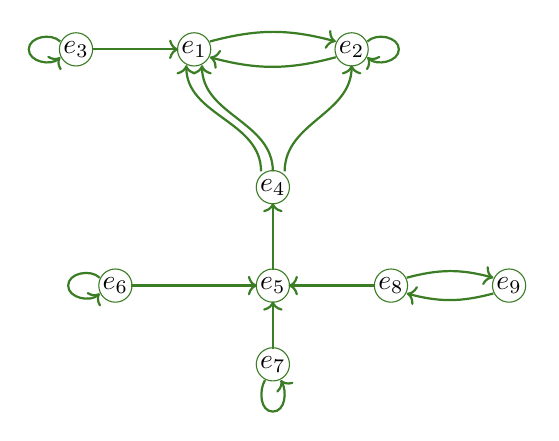
\begin{tikzpicture}[scale = 0.5, color=OliveGreen]
        %% vertex positions
        \coordinate (1) at (-2,9-1); 
        \coordinate (2) at (2,9-1);
        \coordinate (3) at (-5,9-1);
        \coordinate (4) at (0,4.5);
        \coordinate (5) at (0,0+2);
        \coordinate (6) at (-4,0+2);
        \coordinate (7) at (0,-4+4);
        \coordinate (8) at (3,0+2);
        \coordinate (9) at (6,0+2);
        % draw vertices
        \draw[fill=white] \foreach \m in {1,...,9} {
            (\m) circle (12pt) 
            };
        %% label vertices
        \draw \foreach \m in {1,...,9} {
            node[text=black] at (\m) {$e_\m$}
        };
        %%% edges
        \draw[->,thick] (-1.6,9.2-1) to[out=15, in=165] (1.6,9.2-1);
        \draw[<-,thick] (-1.6,8.8-1) to[out=-15, in=-165] (1.6,8.8-1);
        \draw[<-,thick] (2.4,8.8-1) to[out=-45, in=down] (3.2,9-1) to[out=up, in=45] (2.4,9.2-1);
        \draw[->,thick] (-4.6,9-1) to[out=right, in=left] (-2.4,9-1);
        \draw[<-,thick] (-5.4,8.8-1) to[out=-135, in=down] (-6.2,9-1) to[out=up, in=135] (-5.4,9.2-1);
        \draw[->,thick] (-0.3,4.9) to[out=up, in=down] (-2.2,8.6-1);
        \draw[->,thick] (0,4.9) to[out=up, in=down] (-1.8,8.6-1);
        \draw[->,thick] (0.3,4.9) to[out=up, in=down] (2,8.6-1);
        \draw[->,thick] (0,0.4+2) to[out=up, in=down] (0, 4.1);
        \draw[->,thick] (0,-3.6+4) to[out=up, in=down] (0, -0.4+2);
        \draw[<-,thick] (0.2,-4.4+4) to[out=-60, in=right] (0,-5.2+4) to[out=left, in=-120] (-0.2,-4.4+4);
        \draw[->,thick] (-3.6,0+2) to[out=right, in=left] (-0.4,0+2);
        \draw[<-,thick] (-4.4,-0.2+2) to[out=-135, in=down] (-5.2,0+2) to[out=up, in=135] (-4.4,0.2+2);
        \draw[<-,thick] (0.4,0+2) to[out=right, in=left] (2.6,0+2);
        \draw[->,thick] (3.4,0.2+2) to[out=15, in=165] (5.6,0.2+2);
        \draw[<-,thick] (3.4,-0.2+2) to[out=-15, in=-165] (5.6,-0.2+2);
    \end{tikzpicture}
\end{equation}
In the graph above each arrow from $e_j$ to $e_i$ indicates an occurrence of $e_i$ in the decay of $e_j$. For example, since $e_4$ decays into $e_1e_2e_1$ we have one arrow from $e_4$ to $e_2$ and two arrows from $e_4$ to $e_1$. In other words, the number of arrows from $e_j$ to $e_i$ in the decay graph is equal to the $i,j$-entry in the decay matrix (\ref{negafibnary 9x9 decay matrix}). 

Now, looking at the decay graph we see there is a path from each of the nine elements $e_1,\ldots,e_9$ to both $e_1$ and $e_2$. It follows that $e_1$ and $e_2$ occur in any negafibnary look and say sequence whose terms are compounds of $e_1,\ldots,e_9$. Hence, all such look and say sequences grow at rate $\varphi$. 

\begin{exercise}
    Draw the decay graph for the ten elements listed in Exercise \ref{exercise::negabinary periodic table} in the negabinary case. What are the possible growth rates of the negabinary look and say sequences whose terms are eventually compounds of those ten elements? 
\end{exercise}

\subsection{Cosmological Theorems} In this section we will complete our solution to Problem \ref{problem:: cosmological theorem} by providing a Cosmological Theorem for negafibnary look and say sequences (see Theorem \ref{theorem:: negafibnary cosmological theorem}). 
As we have previously mentioned, Conway provided a Cosmological Theorem for standard look and say sequences in \cite{Conway}. However, Conway's proof of his Cosmological Theorem was not included in \cite{Conway} because it involved a ``very subtle and complicated argument, which (almost) reduced the problem to tracking a few hundred cases''. Proofs of Conway's Cosmological Theorem can be found in \cite{Ekhad-Zeilberger} and \cite{Litherland}. In the negafibnary case, we will provide a relatively simple proof. The steps in the proof are broken into lemmas, the first of which shows there is a bound on the number of consecutive 1's appearing in negafibnary look and say sequence:



\begin{lemma}\label{lemma::negafibnary reduction of 1s}
    Suppose $x_0\to x_1\to x_2\to\cdots$ is a negafibnary look and say sequence. Whenever $j>0$, $x_j$ is a compound of elements of the form $1^{m}0^{n}$ with $1\leq m\leq 3$ and $n\geq 0$.
\end{lemma}

\begin{proof}
    If $j>0$, $x_j$ starts with the negafibnary representation of some integer, and thus the first bit in $x_j$ is a 1. Therefore $x_j$ is a compound of elements of the form $1^{m}0^{n}$ with $m\geq 1$ and $n\geq 0$. To show each $m\leq 3$, suppose $B=111$ appears somewhere within $x_j$. Since negafibnary representations cannot have consecutive 1's, the first (resp.~last) 1 in $B$ must be the end (resp.~start) of some negafibnary representation, whence there cannot be another 1 in $x_j$ to the left (resp.~right) of $B$. Thus, there cannot be a run of more than 3 consecutive 1's in $x_j$.
\end{proof}

In order to show the number of consecutive 0's in a negafibnary look and say sequence is bounded, we need a more precise understanding of consecutive 0's in negafibnary representations. Part (3) of the following lemma gives us precisely that:

\begin{lemma}\label{Lemma::negafibnary props}
    Suppose $n$ is an integer with $k$ bits in its negafibnary representation. 
    \begin{enumerate}
        \item If $k$ is odd, then $F_{k-1}< n\leq F_{k+1}$. 

        \item If $k$ is even, then $-F_{k+1}<n\leq -F_{k-1}$. 

        \item If $n>0$ and there is a run of $r$ consecutive 0's in the negafibnary representation of $n$, then $n\geq F_{r+1}$.
    \end{enumerate} 
\end{lemma}

\begin{proof}
    (1) Suppose $k=2\ell + 1$ for some integer $\ell\geq 0$. The maximal negafibnary representation with $k$ bits is obtained by using the maximal number of positive Fibonacci numbers, namely $1010\cdots101=(10)^\ell 1$, which is the negafibnary representation of the integer
    \[\sum_{i=0}^\ell F_{-2i-1} = \sum_{i=0}^\ell \left(F_{-2i} - F_{-2i-2}\right) = F_0-F_{-2\ell-2} = 0-F_{-k-1}=F_{k+1}.\]
    Similarly, we use the maximal number of negative Fibonacci numbers to obtain the minimal $k$-bit negafibnary representation $100(10)^{\ell-1}$, which corresponds to 
    \begin{align*}
        F_{-k}+\sum_{i=1}^{\ell-1} F_{-2i} 
        & = F_{-k}+\sum_{i=1}^{\ell-1} \left(F_{-2i+1} - F_{-2i-1}\right) = F_{-k} + F_{-1}-F_{-2\ell+1} \\
        & = F_{k}+1-F_{2\ell-1} = F_{k}+1-F_{k-2} = 1+F_{k-1}.
    \end{align*}

    (2) The proof is similar to that of (1). Set $k=2\ell$. Then the minimal $k$-bit negafibnary representation is $(10)^\ell$, which corresponds to 
    \begin{align*}
        \sum_{i=1}^{\ell} F_{-2i} 
        & = \sum_{i=1}^{\ell} \left(F_{-2i+1} - F_{-2i-1}\right) = F_{-1} -F_{-2\ell-1} 
         = 1-F_{2\ell+1} = 1-F_{k+1}.
    \end{align*}
    The maximal $k$-bit negafibnary representation is $10(01)^{\ell-1}$, which corresponds to 
    \begin{align*}
        F_{-k}+\sum_{i=1}^{\ell-1} F_{-2i+1} 
        & = F_{-k}+\sum_{i=1}^{\ell-1} \left(F_{-2i+2} - F_{-2i}\right) = F_{-k}+F_{0}-F_{-2\ell+2} \\ 
        & = F_{-k}-F_{-k+2} = -F_{-k+1}  = -F_{k-1}.
    \end{align*}

    (3) Let $n$ denote the minimal positive integer whose negafibnary representation contains a run of at least $r$ consecutive 0's, and let $k$ denote the number of bits in that representation. It follows from (1) and (2) that $k$ will be the smallest odd integer which allows for $r$ consecutive $0$'s. In other words, $k=r+1$ if $r$ is even and $k=r+2$ if $r$ is odd. Moreover, $n$ corresponds to the smallest such $k$-bit representation with $r$ consecutive 0's, namely $10^r$ or $10^{r+1}$. Therefore $n=F_{r+1}$ or $n=F_{r+2}$. In either case, $n\geq F_{r+1}$.
\end{proof}

We are now in position to show that in any negafibnary look and say sequence, the terms will eventually have at most five consecutive 0's:

\begin{lemma}\label{lemma::negafibnary reduction of 0s}
    Suppose the element $1^{m'}0^{n'}$ appears in the negafibnary decay of $1^m0^n$. 
    If $1\leq m\leq 3$ and $n>5$, then $1\leq m'\leq 3$ and $n'<n$.
\end{lemma}

\begin{proof}
    The inequality for $m'$ follows from Lemma \ref{lemma::negafibnary reduction of 1s}. To show the inequality for $n'$, 
    let $a$ and $b$ denote the negafibnary representations of $m$ and $n$ respectively so that $1^m0^n\to a1b0$. Since $1\leq m\leq 3$ we know $a$ is one of $1, 100$, or $101$. Thus, if $1^{m'}0^{n'}$ appears in $a1$ then $n'\leq 2<5<n$. On the other hand, if $1^{m'}0^{n'}$ appears in $b0$, then there must exist a run of at least $n'-1$ consecutive 0's in $b$. Whence $n\geq F_{n'}$ by part (3) of Lemma \ref{Lemma::negafibnary props}. Finally, since $n>5$ we have $F_n>n\geq F_{n'}$, which implies $n>n'$.
\end{proof}


\begin{theorem}\label{theorem:: negafibnary cosmological theorem}
    (Negafibnary Cosmological Theorem)
    The terms of every negafibnary look and say sequence are eventually compounds of the nine elements listed in the negafibnary periodic table (\ref{table:: negafibnary periodic table}). Consequently, every negafibnary look and say sequence grows at the rate $\varphi$.  
\end{theorem}

\begin{proof}
    By Lemma \ref{lemma::negafibnary reduction of 1s} it suffices to show every look and say sequence with seed of the form $1^m0^n$ with $1\leq m\leq 3$ has terms that are eventually compounds of the nine elements listed in the periodic table (\ref{table:: negafibnary periodic table}). We will do so by inducting on $n$. For the base case we consider the 18 seeds $1^m0^n$ with $1\leq m\leq 3$ and $0\leq n\leq 5$. The following decay graph (which extends (\ref{negafibnary decay graph})) summarizes the decay of all 18 elements, completing the base case:
    \begin{equation*}
        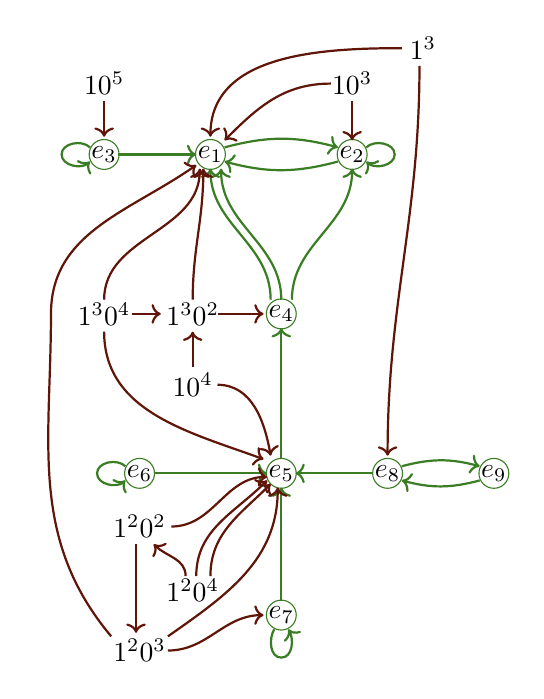
\begin{tikzpicture}[scale = 0.45, color=OliveGreen]
            %% vertex positions
            \coordinate (1) at (-2,9); 
            \coordinate (2) at (2,9);
            \coordinate (3) at (-5,9);
            \coordinate (4) at (0,4.5);
            \coordinate (5) at (0,0);
            \coordinate (6) at (-4,0);
            \coordinate (7) at (0,-4);
            \coordinate (8) at (3,0);
            \coordinate (9) at (6,0);
            % draw vertices
            \draw[fill=white] \foreach \m in {1,...,9} {
                (\m) circle (12pt) 
                };
            %% label vertices
            \draw \foreach \m in {1,...,9} {
                node[text=black] at (\m) {$e_\m$}
            };
            %%% edges
            \draw[->,thick] (-1.6,9.2) to[out=15, in=165] (1.6,9.2);
            \draw[<-,thick] (-1.6,8.8) to[out=-15, in=-165] (1.6,8.8);
            \draw[<-,thick] (2.4,8.8) to[out=-45, in=down] (3.2,9) to[out=up, in=45] (2.4,9.2);
            \draw[->,thick] (-4.6,9) to[out=right, in=left] (-2.4,9);
            \draw[<-,thick] (-5.4,8.8) to[out=-135, in=down] (-6.2,9) to[out=up, in=135] (-5.4,9.2);
            \draw[->,thick] (-0.3,4.9) to[out=up, in=down] (-2,8.6);
            \draw[->,thick] (0,4.9) to[out=up, in=down] (-1.7,8.6);
            \draw[->,thick] (0.3,4.9) to[out=up, in=down] (2,8.6);
            \draw[->,thick] (0,0.4) to[out=up, in=down] (0, 4.1);
            \draw[->,thick] (0,-3.6) to[out=up, in=down] (0, -0.4);
            \draw[<-,thick] (0.2,-4.4) to[out=-60, in=right] (0,-5.2) to[out=left, in=-120] (-0.2,-4.4);
            \draw[->,thick] (-3.6,0) to[out=right, in=left] (-0.4,0);
            \draw[<-,thick] (-4.4,-0.2) to[out=-135, in=down] (-5.2,0) to[out=up, in=135] (-4.4,0.2);
            \draw[<-,thick] (0.4,0) to[out=right, in=left] (2.6,0);
            \draw[->,thick] (3.4,0.2) to[out=15, in=165] (5.6,0.2);
            \draw[<-,thick] (3.4,-0.2) to[out=-15, in=-165] (5.6,-0.2);
            % Other 9 elements:
            \draw node[text=black] at (-2.5,4.5) {$1^30^2$};
            \draw node[text=black] at (-5,4.5) {$1^30^4$};
            \draw node[text=black] at (-2.5,2.5) {$10^4$};
            \draw node[text=black] at (-4,-1.5) {$1^20^2$};
            \draw node[text=black] at (-2.5,-3.3) {$1^20^4$};
            \draw node[text=black] at (-4,-5) {$1^20^3$};
            \draw node[text=black] at (2,11) {$10^3$};
            \draw node[text=black] at (4,12) {$1^3$};
            \draw node[text=black] at (-5,11) {$10^5$};
            \draw[->,thick, color=Sepia] (-1.8,4.5) to[out=right, in=left] (-0.5,4.5);
            \draw[->,thick, color=Sepia] (-4.2,4.5) to[out=right, in=left] (-3.4,4.5);
            \draw[<-,thick, color=Sepia] (-2.5,4) to[out=down, in=up] (-2.5,3);
            \draw[->,thick, color=Sepia] (-1.8,2.5) to[out=right, in=100] (-0.3,0.5);
            \draw[->,thick, color=Sepia] (-5,4) to[out=down, in=160] (-0.5,0.4);
            \draw[->,thick, color=Sepia] (-2.5,4.9) to[out=up, in=down] (-2.2,8.6);
            \draw[->,thick, color=Sepia] (-5,4.9) to[out=up, in=down] (-2.3,8.6);
            \draw[->,thick, color=Sepia] (-2.7,-2.9) to[out=up, in=-45] (-3.6,-2);
            \draw[->,thick, color=Sepia] (-3.1,-1.5) to[out=right, in=left] (-0.4,-0.1);
            \draw[->,thick, color=Sepia] (-4.1,-2) to[out=down, in=up] (-4.1,-4.5);
            \draw[->,thick, color=Sepia] (-2,-2.9) to[out=up, in=-135] (-0.3,-0.3);
            \draw[->,thick, color=Sepia] (-2.4,-2.9) to[out=up, in=-135] (-0.4,-0.2);
            \draw[->,thick, color=Sepia] (-3.2,-4.6) to[out=35, in=down] (-0.1,-0.4);
            \draw[->,thick, color=Sepia] (-3.2,-5) to[out=right, in=left] (-0.5,-4);
            \draw[->,thick, color=Sepia] (-4.8,-4.6) to[out=130, in=down] (-6.5,4.5) to[out=up, in=-145] (-2.4,8.7);
            \draw[->,thick, color=Sepia] (2,10.5) to[out=down, in=up] (2,9.4);
            \draw[->,thick, color=Sepia] (1.4,11) to[out=left, in=45] (-1.6,9.4);
            \draw[->,thick, color=Sepia] (3.4,12) to[out=left, in=up] (-2,9.5);
            \draw[->,thick, color=Sepia] (3.9,11.5) to[out=down, in=up] (3,0.5);
            \draw[->,thick, color=Sepia] (-5,10.5) to[out=down, in=up] (-5,9.5);
        \end{tikzpicture}
    \end{equation*}

    For the inductive step, fix $n>5$ and assume all elements of the form $1^{m'}0^{n'}$ with $1\leq m'\leq 3$ and $0\leq n'<n$ eventually decay in into compounds of the elements in (\ref{table:: negafibnary periodic table}). By Lemma \ref{lemma::negafibnary reduction of 0s}, each $1^m0^n$ with $1\leq m\leq 3$ decays into a compound of such $1^{m'}0^{n'}$'s, and thus $1^m0^n$ eventually decays into the elements in (\ref{table:: negafibnary periodic table}).
\end{proof}

\begin{exercise} 
The goal of this exercise is to prove the following:

\medskip

\noindent \emph{(Negabinary Cosmological Theorem) The terms of every negabinary look and say sequence are eventually compounds of the ten elements listed in Exercise \ref{exercise::negabinary periodic table}.}

\medskip

\noindent The following steps will lead to such a proof:

\begin{enumerate}
    \item Assume $n>0$ has $\ell$ bits in its negabinary representation. Show that $\ell$ is odd so that $\ell=2k+1$ for some integer $k$. Moreover, show $n\geq\dfrac{4^k+2}{3}$.
    \item Assume $m$ and $n$ have negabinary representations $a$ and $b$ respectively so that $1^m0^n\to a1b0$. Now, let $2k_1+1$ and $2k_2+1$ denote the number of bits in $a$ and $b$ respectively, and set $k=\max\{k_1,k_2\}$. Show that the length of $a1b0$ is less than the length of $1^m0^n$ whenever $4k+4<m+n$.
    \item Continuing with the notation of the previous part, use parts (1) and (2) to show that the length of $a1b0$ is less than the length of $1^m0^n$ whenever $4k+4<\dfrac{4^k+2}{3}$.
    \item Show that $4k+4<\dfrac{4^k+2}{3}$ if and only if $k\geq 3$. 
    \item Use the previous parts to show that the length of $a1b0$ is less than the length of $1^m0^n$ whenever $m\geq 22$ or $n\geq 22$.
    \item Write a computer program\footnote{You can write a short python program using the \texttt{look\_and\_say} module.} to show that each of the 462 elements of the form $1^m0^n$ with $1\leq m<22$ and $0\leq n<22$ eventually decays into compounds of the ten elements listed in Exercise \ref{exercise::negabinary periodic table}.
    \item Use the previous two parts to give an inductive proof that every element of the form $1^m0^n$ with $m>0$ and $n\geq 0$ eventually decays into compounds of the ten elements listed in Exercise \ref{exercise::negabinary periodic table}. Explain why this proves The Negabinary Cosmological Theorem. 
\end{enumerate}

\end{exercise}


% \appendix

% \section{Python sessions for negafibnary look and say sequences}

% The purpose of this appendix is to illustrate how the Python module \texttt{look\_and\_say} can be used to perform various computations on look and say sequences. To do so, we will recreate various results on negafibnary look and say sequences. As in Section \ref{section::negafibnary look and say}, we provide exercises on the negabinary case along the way.

% \subsection{Implementing the negafibnary number system} Before introducing 


% \vfill

% \renewcommand{\bibname}{\textsc{references}} 
\bibliographystyle{alphanum}    
\bibliography{references.bib}  

\end{document}